% Options for packages loaded elsewhere
\PassOptionsToPackage{unicode}{hyperref}
\PassOptionsToPackage{hyphens}{url}
\PassOptionsToPackage{dvipsnames,svgnames,x11names}{xcolor}
%
\documentclass[
  letterpaper,
  DIV=11,
  numbers=noendperiod]{scrartcl}

\usepackage{amsmath,amssymb}
\usepackage{lmodern}
\usepackage{iftex}
\ifPDFTeX
  \usepackage[T1]{fontenc}
  \usepackage[utf8]{inputenc}
  \usepackage{textcomp} % provide euro and other symbols
\else % if luatex or xetex
  \usepackage{unicode-math}
  \defaultfontfeatures{Scale=MatchLowercase}
  \defaultfontfeatures[\rmfamily]{Ligatures=TeX,Scale=1}
\fi
% Use upquote if available, for straight quotes in verbatim environments
\IfFileExists{upquote.sty}{\usepackage{upquote}}{}
\IfFileExists{microtype.sty}{% use microtype if available
  \usepackage[]{microtype}
  \UseMicrotypeSet[protrusion]{basicmath} % disable protrusion for tt fonts
}{}
\makeatletter
\@ifundefined{KOMAClassName}{% if non-KOMA class
  \IfFileExists{parskip.sty}{%
    \usepackage{parskip}
  }{% else
    \setlength{\parindent}{0pt}
    \setlength{\parskip}{6pt plus 2pt minus 1pt}}
}{% if KOMA class
  \KOMAoptions{parskip=half}}
\makeatother
\usepackage{xcolor}
\setlength{\emergencystretch}{3em} % prevent overfull lines
\setcounter{secnumdepth}{-\maxdimen} % remove section numbering
% Make \paragraph and \subparagraph free-standing
\ifx\paragraph\undefined\else
  \let\oldparagraph\paragraph
  \renewcommand{\paragraph}[1]{\oldparagraph{#1}\mbox{}}
\fi
\ifx\subparagraph\undefined\else
  \let\oldsubparagraph\subparagraph
  \renewcommand{\subparagraph}[1]{\oldsubparagraph{#1}\mbox{}}
\fi

\usepackage{color}
\usepackage{fancyvrb}
\newcommand{\VerbBar}{|}
\newcommand{\VERB}{\Verb[commandchars=\\\{\}]}
\DefineVerbatimEnvironment{Highlighting}{Verbatim}{commandchars=\\\{\}}
% Add ',fontsize=\small' for more characters per line
\usepackage{framed}
\definecolor{shadecolor}{RGB}{241,243,245}
\newenvironment{Shaded}{\begin{snugshade}}{\end{snugshade}}
\newcommand{\AlertTok}[1]{\textcolor[rgb]{0.68,0.00,0.00}{#1}}
\newcommand{\AnnotationTok}[1]{\textcolor[rgb]{0.37,0.37,0.37}{#1}}
\newcommand{\AttributeTok}[1]{\textcolor[rgb]{0.40,0.45,0.13}{#1}}
\newcommand{\BaseNTok}[1]{\textcolor[rgb]{0.68,0.00,0.00}{#1}}
\newcommand{\BuiltInTok}[1]{\textcolor[rgb]{0.00,0.23,0.31}{#1}}
\newcommand{\CharTok}[1]{\textcolor[rgb]{0.13,0.47,0.30}{#1}}
\newcommand{\CommentTok}[1]{\textcolor[rgb]{0.37,0.37,0.37}{#1}}
\newcommand{\CommentVarTok}[1]{\textcolor[rgb]{0.37,0.37,0.37}{\textit{#1}}}
\newcommand{\ConstantTok}[1]{\textcolor[rgb]{0.56,0.35,0.01}{#1}}
\newcommand{\ControlFlowTok}[1]{\textcolor[rgb]{0.00,0.23,0.31}{#1}}
\newcommand{\DataTypeTok}[1]{\textcolor[rgb]{0.68,0.00,0.00}{#1}}
\newcommand{\DecValTok}[1]{\textcolor[rgb]{0.68,0.00,0.00}{#1}}
\newcommand{\DocumentationTok}[1]{\textcolor[rgb]{0.37,0.37,0.37}{\textit{#1}}}
\newcommand{\ErrorTok}[1]{\textcolor[rgb]{0.68,0.00,0.00}{#1}}
\newcommand{\ExtensionTok}[1]{\textcolor[rgb]{0.00,0.23,0.31}{#1}}
\newcommand{\FloatTok}[1]{\textcolor[rgb]{0.68,0.00,0.00}{#1}}
\newcommand{\FunctionTok}[1]{\textcolor[rgb]{0.28,0.35,0.67}{#1}}
\newcommand{\ImportTok}[1]{\textcolor[rgb]{0.00,0.46,0.62}{#1}}
\newcommand{\InformationTok}[1]{\textcolor[rgb]{0.37,0.37,0.37}{#1}}
\newcommand{\KeywordTok}[1]{\textcolor[rgb]{0.00,0.23,0.31}{#1}}
\newcommand{\NormalTok}[1]{\textcolor[rgb]{0.00,0.23,0.31}{#1}}
\newcommand{\OperatorTok}[1]{\textcolor[rgb]{0.37,0.37,0.37}{#1}}
\newcommand{\OtherTok}[1]{\textcolor[rgb]{0.00,0.23,0.31}{#1}}
\newcommand{\PreprocessorTok}[1]{\textcolor[rgb]{0.68,0.00,0.00}{#1}}
\newcommand{\RegionMarkerTok}[1]{\textcolor[rgb]{0.00,0.23,0.31}{#1}}
\newcommand{\SpecialCharTok}[1]{\textcolor[rgb]{0.37,0.37,0.37}{#1}}
\newcommand{\SpecialStringTok}[1]{\textcolor[rgb]{0.13,0.47,0.30}{#1}}
\newcommand{\StringTok}[1]{\textcolor[rgb]{0.13,0.47,0.30}{#1}}
\newcommand{\VariableTok}[1]{\textcolor[rgb]{0.07,0.07,0.07}{#1}}
\newcommand{\VerbatimStringTok}[1]{\textcolor[rgb]{0.13,0.47,0.30}{#1}}
\newcommand{\WarningTok}[1]{\textcolor[rgb]{0.37,0.37,0.37}{\textit{#1}}}

\providecommand{\tightlist}{%
  \setlength{\itemsep}{0pt}\setlength{\parskip}{0pt}}\usepackage{longtable,booktabs,array}
\usepackage{calc} % for calculating minipage widths
% Correct order of tables after \paragraph or \subparagraph
\usepackage{etoolbox}
\makeatletter
\patchcmd\longtable{\par}{\if@noskipsec\mbox{}\fi\par}{}{}
\makeatother
% Allow footnotes in longtable head/foot
\IfFileExists{footnotehyper.sty}{\usepackage{footnotehyper}}{\usepackage{footnote}}
\makesavenoteenv{longtable}
\usepackage{graphicx}
\makeatletter
\def\maxwidth{\ifdim\Gin@nat@width>\linewidth\linewidth\else\Gin@nat@width\fi}
\def\maxheight{\ifdim\Gin@nat@height>\textheight\textheight\else\Gin@nat@height\fi}
\makeatother
% Scale images if necessary, so that they will not overflow the page
% margins by default, and it is still possible to overwrite the defaults
% using explicit options in \includegraphics[width, height, ...]{}
\setkeys{Gin}{width=\maxwidth,height=\maxheight,keepaspectratio}
% Set default figure placement to htbp
\makeatletter
\def\fps@figure{htbp}
\makeatother

\KOMAoption{captions}{tableheading}
\makeatletter
\makeatother
\makeatletter
\makeatother
\makeatletter
\@ifpackageloaded{caption}{}{\usepackage{caption}}
\AtBeginDocument{%
\ifdefined\contentsname
  \renewcommand*\contentsname{Table of contents}
\else
  \newcommand\contentsname{Table of contents}
\fi
\ifdefined\listfigurename
  \renewcommand*\listfigurename{List of Figures}
\else
  \newcommand\listfigurename{List of Figures}
\fi
\ifdefined\listtablename
  \renewcommand*\listtablename{List of Tables}
\else
  \newcommand\listtablename{List of Tables}
\fi
\ifdefined\figurename
  \renewcommand*\figurename{Figure}
\else
  \newcommand\figurename{Figure}
\fi
\ifdefined\tablename
  \renewcommand*\tablename{Table}
\else
  \newcommand\tablename{Table}
\fi
}
\@ifpackageloaded{float}{}{\usepackage{float}}
\floatstyle{ruled}
\@ifundefined{c@chapter}{\newfloat{codelisting}{h}{lop}}{\newfloat{codelisting}{h}{lop}[chapter]}
\floatname{codelisting}{Listing}
\newcommand*\listoflistings{\listof{codelisting}{List of Listings}}
\makeatother
\makeatletter
\@ifpackageloaded{caption}{}{\usepackage{caption}}
\@ifpackageloaded{subcaption}{}{\usepackage{subcaption}}
\makeatother
\makeatletter
\@ifpackageloaded{tcolorbox}{}{\usepackage[many]{tcolorbox}}
\makeatother
\makeatletter
\@ifundefined{shadecolor}{\definecolor{shadecolor}{rgb}{.97, .97, .97}}
\makeatother
\makeatletter
\makeatother
\ifLuaTeX
  \usepackage{selnolig}  % disable illegal ligatures
\fi
\IfFileExists{bookmark.sty}{\usepackage{bookmark}}{\usepackage{hyperref}}
\IfFileExists{xurl.sty}{\usepackage{xurl}}{} % add URL line breaks if available
\urlstyle{same} % disable monospaced font for URLs
\hypersetup{
  pdftitle={Lista de exercícios - Amostragem},
  pdfauthor={Gabriel de Jesus Pereira},
  colorlinks=true,
  linkcolor={blue},
  filecolor={Maroon},
  citecolor={Blue},
  urlcolor={Blue},
  pdfcreator={LaTeX via pandoc}}

\title{Lista de exercícios - Amostragem}
\author{Gabriel de Jesus Pereira}
\date{}

\begin{document}
\maketitle
\ifdefined\Shaded\renewenvironment{Shaded}{\begin{tcolorbox}[breakable, interior hidden, enhanced, borderline west={3pt}{0pt}{shadecolor}, boxrule=0pt, sharp corners, frame hidden]}{\end{tcolorbox}}\fi

\hypertarget{pacotes}{%
\subsection{Pacotes}\label{pacotes}}

\begin{Shaded}
\begin{Highlighting}[]
\FunctionTok{library}\NormalTok{(dplyr)}
\end{Highlighting}
\end{Shaded}

\begin{verbatim}

Attaching package: 'dplyr'
\end{verbatim}

\begin{verbatim}
The following objects are masked from 'package:stats':

    filter, lag
\end{verbatim}

\begin{verbatim}
The following objects are masked from 'package:base':

    intersect, setdiff, setequal, union
\end{verbatim}

\begin{Shaded}
\begin{Highlighting}[]
\FunctionTok{library}\NormalTok{(knitr)}
\FunctionTok{library}\NormalTok{(ggplot2)}
\end{Highlighting}
\end{Shaded}

\hypertarget{funuxe7uxe3o-para-questuxf5es-3-e-4}{%
\subsection{Função para questões 3 e
4}\label{funuxe7uxe3o-para-questuxf5es-3-e-4}}

\begin{Shaded}
\begin{Highlighting}[]
\NormalTok{MetricasDados }\OtherTok{\textless{}{-}} \ControlFlowTok{function}\NormalTok{(dados, N, }\AttributeTok{xu =} \ConstantTok{NA}\NormalTok{, }\AttributeTok{tx =} \ConstantTok{NA}\NormalTok{, }\AttributeTok{alpha =} \FloatTok{0.5}\NormalTok{) \{}
\NormalTok{  n }\OtherTok{\textless{}{-}} \FunctionTok{nrow}\NormalTok{(dados)}
\NormalTok{  B }\OtherTok{\textless{}{-}}  \FunctionTok{mean}\NormalTok{(dados[[}\DecValTok{2}\NormalTok{]])}\SpecialCharTok{/}\FunctionTok{mean}\NormalTok{(dados[[}\DecValTok{1}\NormalTok{]])}
\NormalTok{  se }\OtherTok{\textless{}{-}} \FunctionTok{var}\NormalTok{(dados[[}\DecValTok{2}\NormalTok{]] }\SpecialCharTok{{-}}\NormalTok{ B}\SpecialCharTok{*}\NormalTok{dados[[}\DecValTok{1}\NormalTok{]])}
\NormalTok{  t }\OtherTok{\textless{}{-}} \FunctionTok{qt}\NormalTok{(}\DecValTok{1} \SpecialCharTok{{-}}\NormalTok{ alpha}\SpecialCharTok{/}\DecValTok{2}\NormalTok{, }\AttributeTok{df =}\NormalTok{ n }\SpecialCharTok{{-}} \DecValTok{1}\NormalTok{)}
  \FunctionTok{tibble}\NormalTok{(}
    \StringTok{\textasciigrave{}}\AttributeTok{Estimador média AAS}\StringTok{\textasciigrave{}} \OtherTok{=} \FunctionTok{mean}\NormalTok{(dados[[}\DecValTok{2}\NormalTok{]]),}
    \StringTok{\textasciigrave{}}\AttributeTok{Variância média AAS}\StringTok{\textasciigrave{}} \OtherTok{=}\NormalTok{ (}\DecValTok{1} \SpecialCharTok{{-}}\NormalTok{ n}\SpecialCharTok{/}\NormalTok{N)}\SpecialCharTok{*}\FunctionTok{var}\NormalTok{(dados[[}\DecValTok{2}\NormalTok{]])}\SpecialCharTok{/}\NormalTok{n,}
    \StringTok{\textasciigrave{}}\AttributeTok{Estimador média razão}\StringTok{\textasciigrave{}} \OtherTok{=}\NormalTok{ B}\SpecialCharTok{*}\NormalTok{xu,}
    \StringTok{\textasciigrave{}}\AttributeTok{Variância média razão}\StringTok{\textasciigrave{}} \OtherTok{=}\NormalTok{ (}\DecValTok{1} \SpecialCharTok{{-}}\NormalTok{ n}\SpecialCharTok{/}\NormalTok{N)}\SpecialCharTok{*}\NormalTok{(xu}\SpecialCharTok{/}\FunctionTok{mean}\NormalTok{(dados[[}\DecValTok{1}\NormalTok{]]))}\SpecialCharTok{\^{}}\DecValTok{2}\SpecialCharTok{*}\NormalTok{se}\SpecialCharTok{/}\NormalTok{n,}
    \StringTok{\textasciigrave{}}\AttributeTok{Total AAS}\StringTok{\textasciigrave{}} \OtherTok{=}\NormalTok{ N}\SpecialCharTok{*}\FunctionTok{mean}\NormalTok{(dados[[}\DecValTok{2}\NormalTok{]]),}
    \StringTok{\textasciigrave{}}\AttributeTok{Variância total AAS}\StringTok{\textasciigrave{}} \OtherTok{=}\NormalTok{ N}\SpecialCharTok{\^{}}\DecValTok{2}\SpecialCharTok{*}\NormalTok{(}\DecValTok{1} \SpecialCharTok{{-}}\NormalTok{ n}\SpecialCharTok{/}\NormalTok{N)}\SpecialCharTok{*}\FunctionTok{var}\NormalTok{(dados[[}\DecValTok{2}\NormalTok{]])}\SpecialCharTok{/}\NormalTok{n,}
    \StringTok{\textasciigrave{}}\AttributeTok{Total razão}\StringTok{\textasciigrave{}} \OtherTok{=}\NormalTok{ B}\SpecialCharTok{*}\NormalTok{tx,}
    \StringTok{\textasciigrave{}}\AttributeTok{Variância total razão}\StringTok{\textasciigrave{}} \OtherTok{=}\NormalTok{ (}\DecValTok{1} \SpecialCharTok{{-}}\NormalTok{ n}\SpecialCharTok{/}\NormalTok{N)}\SpecialCharTok{*}\NormalTok{(tx}\SpecialCharTok{/}\FunctionTok{mean}\NormalTok{(dados[[}\DecValTok{1}\NormalTok{]]))}\SpecialCharTok{\^{}}\DecValTok{2}\SpecialCharTok{*}\NormalTok{se}\SpecialCharTok{/}\NormalTok{n,}
    \StringTok{\textasciigrave{}}\AttributeTok{IC para média AAS}\StringTok{\textasciigrave{}} \OtherTok{=} \FunctionTok{list}\NormalTok{(}\StringTok{\textasciigrave{}}\AttributeTok{Estimador média AAS}\StringTok{\textasciigrave{}} \SpecialCharTok{+} \FunctionTok{c}\NormalTok{(}\SpecialCharTok{{-}}\NormalTok{t }\SpecialCharTok{*} \FunctionTok{sqrt}\NormalTok{(}\StringTok{\textasciigrave{}}\AttributeTok{Variância média AAS}\StringTok{\textasciigrave{}}\NormalTok{), t }\SpecialCharTok{*} \FunctionTok{sqrt}\NormalTok{(}\StringTok{\textasciigrave{}}\AttributeTok{Variância média AAS}\StringTok{\textasciigrave{}}\NormalTok{))),}
    \StringTok{\textasciigrave{}}\AttributeTok{IC para média razão}\StringTok{\textasciigrave{}} \OtherTok{=} \FunctionTok{list}\NormalTok{(}\StringTok{\textasciigrave{}}\AttributeTok{Estimador média razão}\StringTok{\textasciigrave{}} \SpecialCharTok{+} \FunctionTok{c}\NormalTok{(}\SpecialCharTok{{-}}\NormalTok{t }\SpecialCharTok{*} \FunctionTok{sqrt}\NormalTok{(}\StringTok{\textasciigrave{}}\AttributeTok{Variância média razão}\StringTok{\textasciigrave{}}\NormalTok{), t }\SpecialCharTok{*} \FunctionTok{sqrt}\NormalTok{(}\StringTok{\textasciigrave{}}\AttributeTok{Variância média razão}\StringTok{\textasciigrave{}}\NormalTok{))),}
    \StringTok{\textasciigrave{}}\AttributeTok{IC para total AAS}\StringTok{\textasciigrave{}} \OtherTok{=} \FunctionTok{list}\NormalTok{(}\StringTok{\textasciigrave{}}\AttributeTok{Total AAS}\StringTok{\textasciigrave{}} \SpecialCharTok{+} \FunctionTok{c}\NormalTok{(}\SpecialCharTok{{-}}\NormalTok{t}\SpecialCharTok{*}\FunctionTok{sqrt}\NormalTok{(}\StringTok{\textasciigrave{}}\AttributeTok{Variância total AAS}\StringTok{\textasciigrave{}}\NormalTok{), t}\SpecialCharTok{*}\FunctionTok{sqrt}\NormalTok{(}\StringTok{\textasciigrave{}}\AttributeTok{Variância total AAS}\StringTok{\textasciigrave{}}\NormalTok{))),}
    \StringTok{\textasciigrave{}}\AttributeTok{IC para total razão}\StringTok{\textasciigrave{}} \OtherTok{=} \FunctionTok{list}\NormalTok{(}\StringTok{\textasciigrave{}}\AttributeTok{Total razão}\StringTok{\textasciigrave{}} \SpecialCharTok{+} \FunctionTok{c}\NormalTok{(}\SpecialCharTok{{-}}\NormalTok{t}\SpecialCharTok{*}\FunctionTok{sqrt}\NormalTok{(}\StringTok{\textasciigrave{}}\AttributeTok{Variância total razão}\StringTok{\textasciigrave{}}\NormalTok{), t}\SpecialCharTok{*}\FunctionTok{sqrt}\NormalTok{(}\StringTok{\textasciigrave{}}\AttributeTok{Variância total razão}\StringTok{\textasciigrave{}}\NormalTok{)))}
\NormalTok{  ) }
\NormalTok{\}}
\end{Highlighting}
\end{Shaded}

\hypertarget{questuxe3o-3}{%
\subsection{Questão 3}\label{questuxe3o-3}}

\begin{Shaded}
\begin{Highlighting}[]
\CommentTok{\# Banco de Dados}

\NormalTok{Banco3 }\OtherTok{\textless{}{-}} \FunctionTok{tibble}\NormalTok{(}
  \AttributeTok{X =} \FunctionTok{c}\NormalTok{(}\DecValTok{12}\NormalTok{, }\DecValTok{11}\NormalTok{, }\DecValTok{8}\NormalTok{, }\DecValTok{9}\NormalTok{, }\DecValTok{11}\NormalTok{, }\DecValTok{8}\NormalTok{, }\DecValTok{7}\NormalTok{, }\DecValTok{10}\NormalTok{, }\DecValTok{12}\NormalTok{, }\DecValTok{11}\NormalTok{, }\DecValTok{6}\NormalTok{, }\DecValTok{8}\NormalTok{, }\DecValTok{10}\NormalTok{, }\DecValTok{12}\NormalTok{, }\DecValTok{9}\NormalTok{, }\DecValTok{9}\NormalTok{, }\DecValTok{7}\NormalTok{, }\DecValTok{11}\NormalTok{, }\DecValTok{9}\NormalTok{, }\DecValTok{8}\NormalTok{),}
  \AttributeTok{Y =} \FunctionTok{c}\NormalTok{(}\DecValTok{125}\NormalTok{, }\DecValTok{119}\NormalTok{, }\DecValTok{83}\NormalTok{, }\DecValTok{85}\NormalTok{, }\DecValTok{99}\NormalTok{, }\DecValTok{117}\NormalTok{, }\DecValTok{69}\NormalTok{, }\DecValTok{133}\NormalTok{, }\DecValTok{154}\NormalTok{, }\DecValTok{168}\NormalTok{, }\DecValTok{61}\NormalTok{, }\DecValTok{80}\NormalTok{, }\DecValTok{114}\NormalTok{, }\DecValTok{147}\NormalTok{, }\DecValTok{122}\NormalTok{, }\DecValTok{106}\NormalTok{, }\DecValTok{82}\NormalTok{, }\DecValTok{88}\NormalTok{, }\DecValTok{97}\NormalTok{, }\DecValTok{99}\NormalTok{)}
\NormalTok{                 )}
\end{Highlighting}
\end{Shaded}

\hypertarget{a}{%
\subsubsection{a)}\label{a}}

\begin{Shaded}
\begin{Highlighting}[]
\NormalTok{Banco3 }\SpecialCharTok{|\textgreater{}} 
  \FunctionTok{ggplot}\NormalTok{() }\SpecialCharTok{+}
  \FunctionTok{geom\_point}\NormalTok{(}\FunctionTok{aes}\NormalTok{(}\AttributeTok{x =}\NormalTok{ X, }\AttributeTok{y =}\NormalTok{ Y))}
\end{Highlighting}
\end{Shaded}

\begin{figure}[H]

{\centering 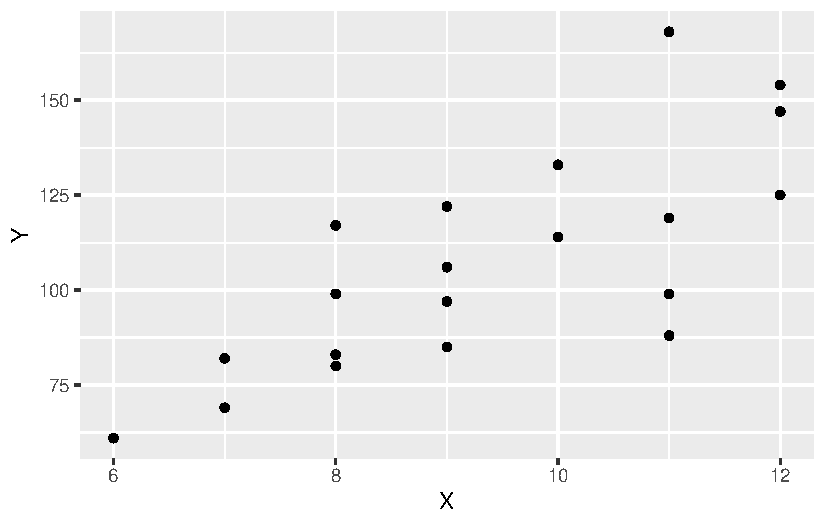
\includegraphics{trabalho_amostragem_files/figure-pdf/unnamed-chunk-4-1.pdf}

}

\end{figure}

\begin{Shaded}
\begin{Highlighting}[]
\CommentTok{\# Coeficiente de correlação}

\FunctionTok{kable}\NormalTok{(}\FunctionTok{cor}\NormalTok{(Banco3))}
\end{Highlighting}
\end{Shaded}

\begin{longtable}[]{@{}lrr@{}}
\toprule()
& X & Y \\
\midrule()
\endhead
X & 1.0000000 & 0.7573225 \\
Y & 0.7573225 & 1.0000000 \\
\bottomrule()
\end{longtable}

\hypertarget{b-c-e-d}{%
\subsubsection{b), c) e d)}\label{b-c-e-d}}

\begin{Shaded}
\begin{Highlighting}[]
\NormalTok{df1 }\OtherTok{\textless{}{-}} \FunctionTok{MetricasDados}\NormalTok{(Banco3, }\AttributeTok{N =} \DecValTok{1132}\NormalTok{, }\AttributeTok{xu =} \DecValTok{10}\NormalTok{) }\SpecialCharTok{|\textgreater{}} 
  \FunctionTok{select\_if}\NormalTok{(}\SpecialCharTok{\textasciitilde{}} \SpecialCharTok{!}\FunctionTok{any}\NormalTok{(}\FunctionTok{is.na}\NormalTok{(.))) }\SpecialCharTok{|\textgreater{}}
  \FunctionTok{select}\NormalTok{(}\SpecialCharTok{{-}}\FunctionTok{contains}\NormalTok{(}\FunctionTok{c}\NormalTok{(}\StringTok{"total"}\NormalTok{, }\StringTok{"Variância"}\NormalTok{)))}
\FunctionTok{kable}\NormalTok{(df1)}
\end{Highlighting}
\end{Shaded}

\begin{longtable}[]{@{}
  >{\raggedleft\arraybackslash}p{(\columnwidth - 6\tabcolsep) * \real{0.2469}}
  >{\raggedleft\arraybackslash}p{(\columnwidth - 6\tabcolsep) * \real{0.2716}}
  >{\raggedright\arraybackslash}p{(\columnwidth - 6\tabcolsep) * \real{0.2346}}
  >{\raggedright\arraybackslash}p{(\columnwidth - 6\tabcolsep) * \real{0.2469}}@{}}
\toprule()
\begin{minipage}[b]{\linewidth}\raggedleft
Estimador média AAS
\end{minipage} & \begin{minipage}[b]{\linewidth}\raggedleft
Estimador média razão
\end{minipage} & \begin{minipage}[b]{\linewidth}\raggedright
IC para média AAS
\end{minipage} & \begin{minipage}[b]{\linewidth}\raggedright
IC para média razão
\end{minipage} \\
\midrule()
\endhead
107.4 & 114.2553 & 103.0321, 111.7679 & 111.2171, 117.2936 \\
\bottomrule()
\end{longtable}

\hypertarget{e}{%
\subsubsection{e)}\label{e}}

\hypertarget{f}{%
\subsubsection{f)}\label{f}}

\hypertarget{questuxe3o-4}{%
\subsection{Questão 4}\label{questuxe3o-4}}

\begin{Shaded}
\begin{Highlighting}[]
\CommentTok{\# Banco de dados para a questão 4}
\NormalTok{Banco4 }\OtherTok{\textless{}{-}} \FunctionTok{tibble}\NormalTok{(}\AttributeTok{X =} \FunctionTok{c}\NormalTok{(}\DecValTok{12}\NormalTok{, }\DecValTok{30}\NormalTok{, }\DecValTok{24}\NormalTok{, }\DecValTok{24}\NormalTok{, }\DecValTok{18}\NormalTok{, }\DecValTok{30}\NormalTok{, }\DecValTok{12}\NormalTok{, }\DecValTok{6}\NormalTok{, }\DecValTok{36}\NormalTok{, }\DecValTok{42}\NormalTok{),}
                 \AttributeTok{Y =} \FunctionTok{c}\NormalTok{(}\DecValTok{18}\NormalTok{, }\DecValTok{42}\NormalTok{, }\DecValTok{24}\NormalTok{, }\DecValTok{36}\NormalTok{, }\DecValTok{24}\NormalTok{, }\DecValTok{36}\NormalTok{, }\DecValTok{14}\NormalTok{, }\DecValTok{10}\NormalTok{, }\DecValTok{48}\NormalTok{, }\DecValTok{54}\NormalTok{))}
\end{Highlighting}
\end{Shaded}

\hypertarget{a-1}{%
\subsubsection{a)}\label{a-1}}

\begin{Shaded}
\begin{Highlighting}[]
\NormalTok{Banco4 }\SpecialCharTok{|\textgreater{}}
  \FunctionTok{ggplot}\NormalTok{() }\SpecialCharTok{+}
  \FunctionTok{geom\_point}\NormalTok{(}\FunctionTok{aes}\NormalTok{(}\AttributeTok{x =}\NormalTok{ X, }\AttributeTok{y =}\NormalTok{ Y))}
\end{Highlighting}
\end{Shaded}

\begin{figure}[H]

{\centering 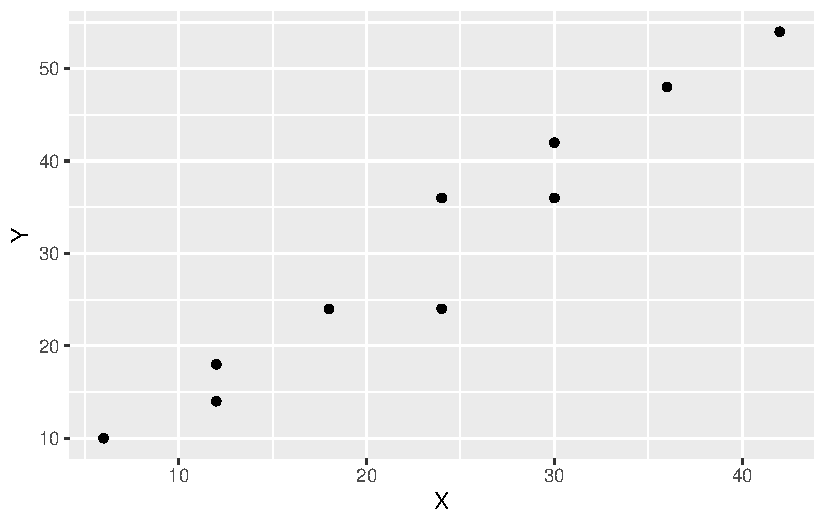
\includegraphics{trabalho_amostragem_files/figure-pdf/unnamed-chunk-8-1.pdf}

}

\end{figure}

\begin{Shaded}
\begin{Highlighting}[]
\FunctionTok{kable}\NormalTok{(}\FunctionTok{cor}\NormalTok{(Banco4))}
\end{Highlighting}
\end{Shaded}

\begin{longtable}[]{@{}lrr@{}}
\toprule()
& X & Y \\
\midrule()
\endhead
X & 1.0000000 & 0.9729456 \\
Y & 0.9729456 & 1.0000000 \\
\bottomrule()
\end{longtable}

\hypertarget{b-c-d-e-e}{%
\subsubsection{b), c), d) e e)}\label{b-c-d-e-e}}

\begin{Shaded}
\begin{Highlighting}[]
\NormalTok{df2 }\OtherTok{\textless{}{-}} \FunctionTok{MetricasDados}\NormalTok{(Banco4, }\AttributeTok{N =} \DecValTok{200}\NormalTok{, }\AttributeTok{tx =} \DecValTok{15600}\NormalTok{) }\SpecialCharTok{|\textgreater{}} 
  \FunctionTok{select\_if}\NormalTok{(}\SpecialCharTok{\textasciitilde{}} \SpecialCharTok{!}\FunctionTok{any}\NormalTok{(}\FunctionTok{is.na}\NormalTok{(.))) }\SpecialCharTok{|\textgreater{}} 
  \FunctionTok{select}\NormalTok{(}\SpecialCharTok{{-}}\FunctionTok{contains}\NormalTok{(}\FunctionTok{c}\NormalTok{(}\StringTok{"média razão"}\NormalTok{, }\StringTok{"Total AAS"}\NormalTok{, }\StringTok{"total AAS"}\NormalTok{)))}
\FunctionTok{kable}\NormalTok{(df2)}
\end{Highlighting}
\end{Shaded}

\begin{longtable}[]{@{}
  >{\raggedleft\arraybackslash}p{(\columnwidth - 10\tabcolsep) * \real{0.1770}}
  >{\raggedleft\arraybackslash}p{(\columnwidth - 10\tabcolsep) * \real{0.1770}}
  >{\raggedleft\arraybackslash}p{(\columnwidth - 10\tabcolsep) * \real{0.1062}}
  >{\raggedleft\arraybackslash}p{(\columnwidth - 10\tabcolsep) * \real{0.1947}}
  >{\raggedright\arraybackslash}p{(\columnwidth - 10\tabcolsep) * \real{0.1681}}
  >{\raggedright\arraybackslash}p{(\columnwidth - 10\tabcolsep) * \real{0.1770}}@{}}
\toprule()
\begin{minipage}[b]{\linewidth}\raggedleft
Estimador média AAS
\end{minipage} & \begin{minipage}[b]{\linewidth}\raggedleft
Variância média AAS
\end{minipage} & \begin{minipage}[b]{\linewidth}\raggedleft
Total razão
\end{minipage} & \begin{minipage}[b]{\linewidth}\raggedleft
Variância total razão
\end{minipage} & \begin{minipage}[b]{\linewidth}\raggedright
IC para média AAS
\end{minipage} & \begin{minipage}[b]{\linewidth}\raggedright
IC para total razão
\end{minipage} \\
\midrule()
\endhead
30.6 & 20.94644 & 20400 & 509886.8 & 27.38383, 33.81617 & 19898.21,
20901.79 \\
\bottomrule()
\end{longtable}

\hypertarget{f-g-e-h}{%
\subsubsection{f), g) e h)}\label{f-g-e-h}}



\end{document}
